\documentclass[a4paper, 12pt]{article}

%\usepackage{cmap}
\usepackage[T2A]{fontenc}
\usepackage[utf8]{inputenc}
\usepackage[english, russian]{babel}
\usepackage{graphicx}
\usepackage[top=1in, bottom=1in, left=3.2cm, right=2.6cm]{geometry}
\graphicspath{./}
\usepackage{biblatex}
\addbibresource{lib.bib}
\linespread{1.5}

\usepackage{listings}
\usepackage{color}


\begin{document}
	
\begin{titlepage}
	\fontsize{12pt}{12pt}\selectfont
	\begin{figure}[t!]
		\centering
		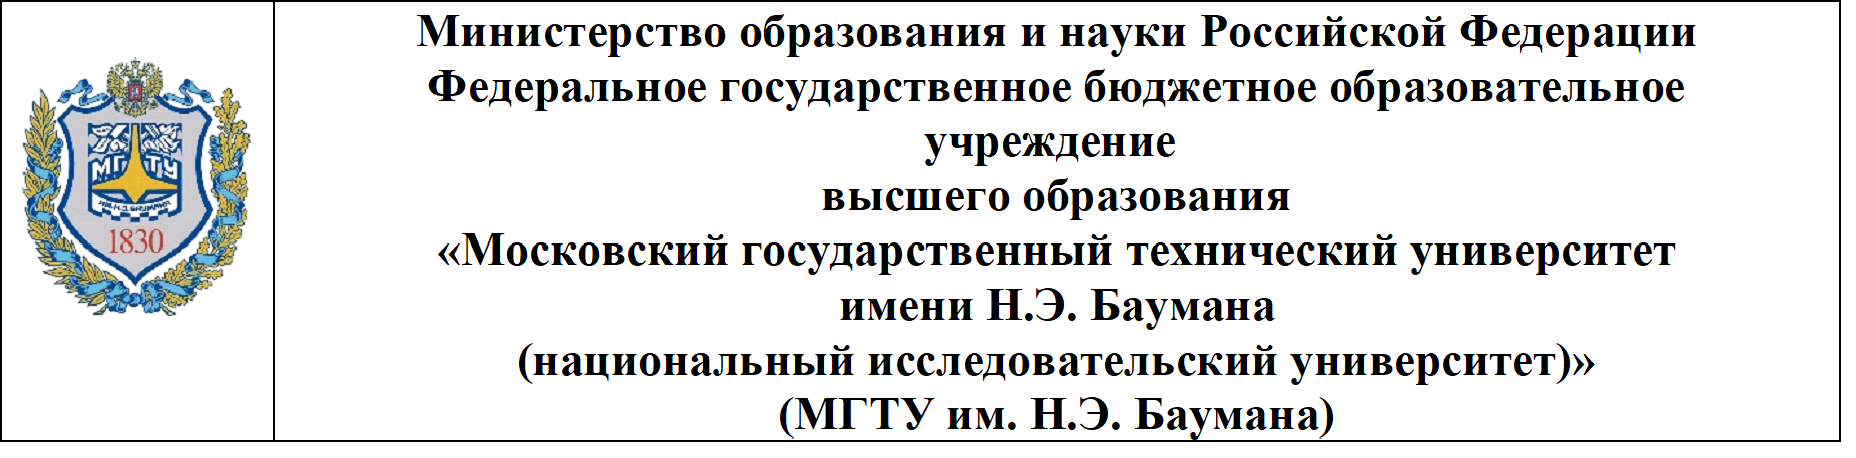
\includegraphics[scale=0.8]{bmstu}
	\end{figure}
	
	\noindent\rule{15cm}{3pt}
	\newline\newline
	\noindent 
	ФАКУЛЬТЕТ 
	\underline{«Информатика и системы управления»} \newline\newline
	
	\noindent КАФЕДРА \underline{«Программное обеспечение ЭВМ и информационные технологии»}\newline\newline\newline\newline\newline\newline
	
	\centering {\LARGE \bf Домашнее задание № 1}
	\vspace{3mm}
	
	\centering {\LARGE По курсу "Анализ Алгоритмов"}

	
	
	\begin{flushright}
		\vspace*{2cm}
		{\large	Студент:\\ Турсунов Жасурбек Рустамович \\ Группа: ИУ7-56Б
			\vspace{5mm}
			\\Преподователи: \\ Волкова Лилия Леонидовна \\ Строганов Юрий Владимирович}
	\end{flushright}
	
	\begin{center}
		\vfill
		Москва, \the\year
		~г.
	\end{center}
\end{titlepage}

\tableofcontents
\clearpage
\newpage


\section{Технологическая часть}
\begin{flushleft} 
	\subsection{Листинг кода}
	В данном пункте представлен листинг кода, функции умножения матриц по Винограду:
	\definecolor{codegreen}{rgb}{0,0.6,0}
	\definecolor{codegray}{rgb}{0.5,0.5,0.5}
	\definecolor{codepurple}{rgb}{0.58,0,0.82}
	\definecolor{backcolour}{rgb}{0.95,0.95,0.92}

	\lstdefinestyle{mystyle}{
		backgroundcolor=\color{backcolour},   
		commentstyle=\color{codegreen},
		keywordstyle=\color{magenta},
		numberstyle=\tiny\color{codegray},
		stringstyle=\color{codepurple},
		basicstyle=\ttfamily\footnotesize,
		breakatwhitespace=false,         
		breaklines=false,                 
		captionpos=b,                    
		keepspaces=true,                 
		numbers=left,                    
		numbersep=5pt,                  
		showspaces=false,                
		showstringspaces=false,
		showtabs=false,                  
		tabsize=4
	}

	\lstset{style=mystyle}

	\begin{lstlisting}[language=Python, caption = Умножение матриц по Винограду]
	for i in range(0, N1):                                      (1)
		for j in range(0, M1/2):								(2)	
			rows[i] += matr1[i][j*2] * matr1[i][j*2+1]			(3)
	for i in range(0, M2):										(4)	
		for j in range(0, N2/2):								(5)
			cols[i] += matr1[j*2][i] * matr1[j*2+1][i]			(6)
	for i in range(0, N1):										(7)
		for j in range(0, M2):									(8)
			res[i][j] = -rows[i] - cols[j]						(9)
			for k in range(0, M1/2):							(10)
				res[i][j] += (matr1[i][2*k+1] + matr2[2*k][j]) *
							 (matr1[i][2*k] + matr2[2*k+1][j])	(11)
	if M1 % 2:													(12)
		for i in range(0, N1):									(13)
			for j in range(0, M2):								(14)
				res[i][j] += matr1[i][M1-1] * matr2[M1-1][j]	(15)
	\end{lstlisting}
	
\end{flushleft}
\clearpage
\newpage
\section{Модели программ}
\subsection{Граф управления программы}
\begin{figure}[h!]
	\centering
	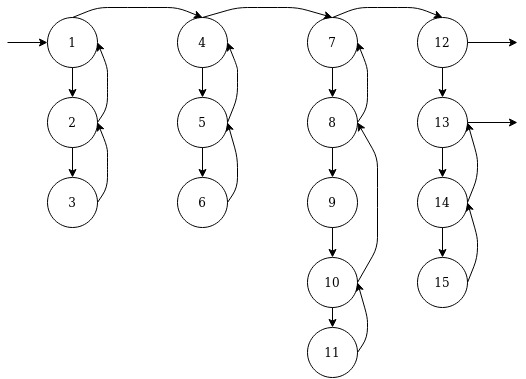
\includegraphics[scale=0.5]{control_graph}
	\caption{Граф управления программы}
\end{figure}

\subsection{Информационный граф программы}
\begin{figure}[h!]
	\centering
	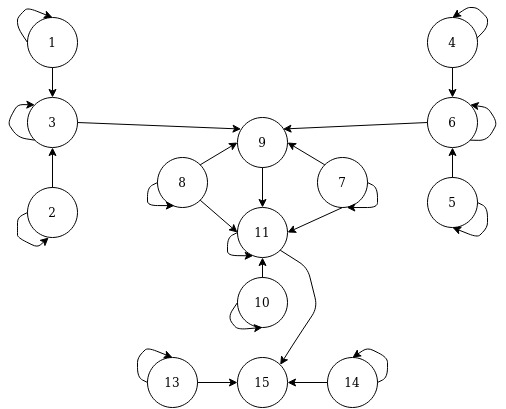
\includegraphics[scale=0.5]{info_graph}
	\caption{Информационный граф программы}
\end{figure}

\clearpage
\newpage
\subsection{Операционная история программы}
\begin{figure}[h!]
	\centering
	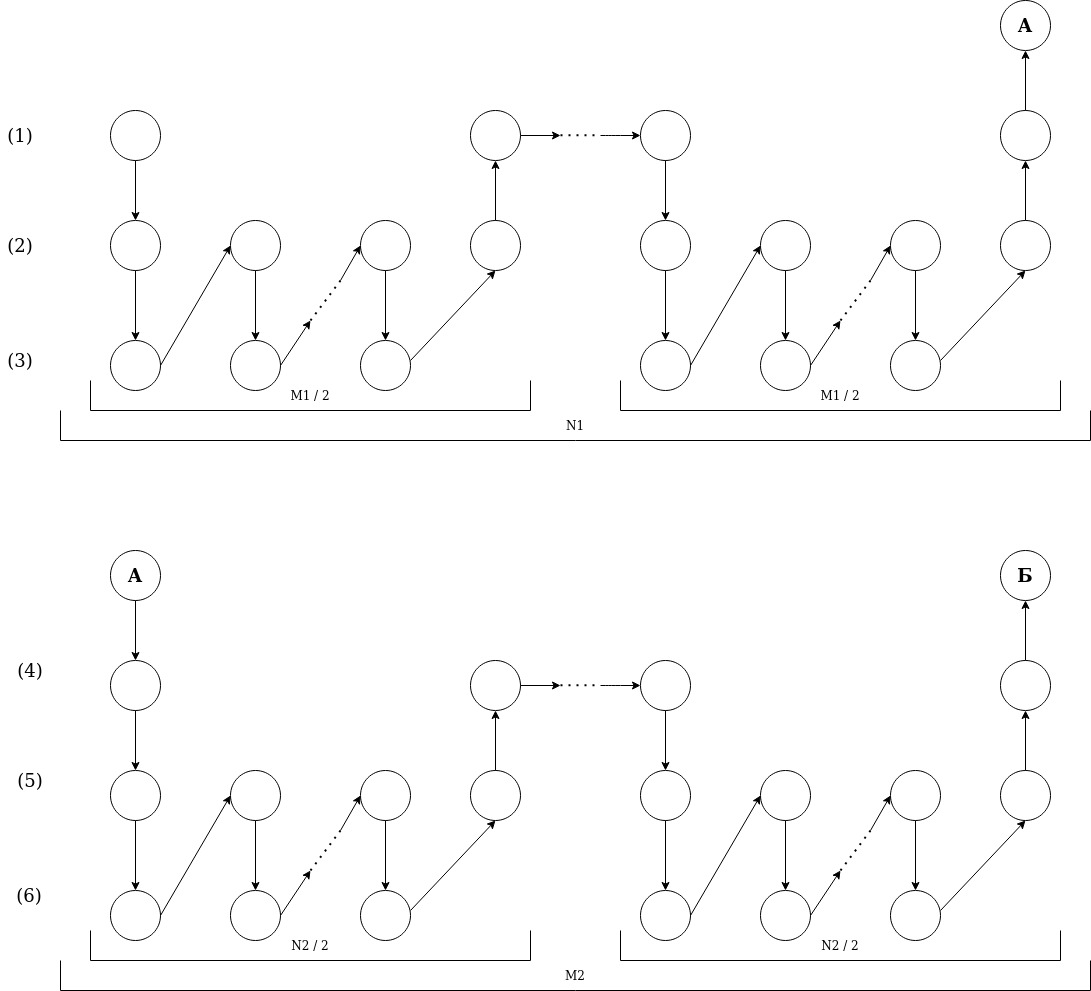
\includegraphics[scale=0.3]{oper_history_1}
	\caption{Операционная история программы. Часть 1}
\end{figure}
\begin{figure}[h!]
	\centering
	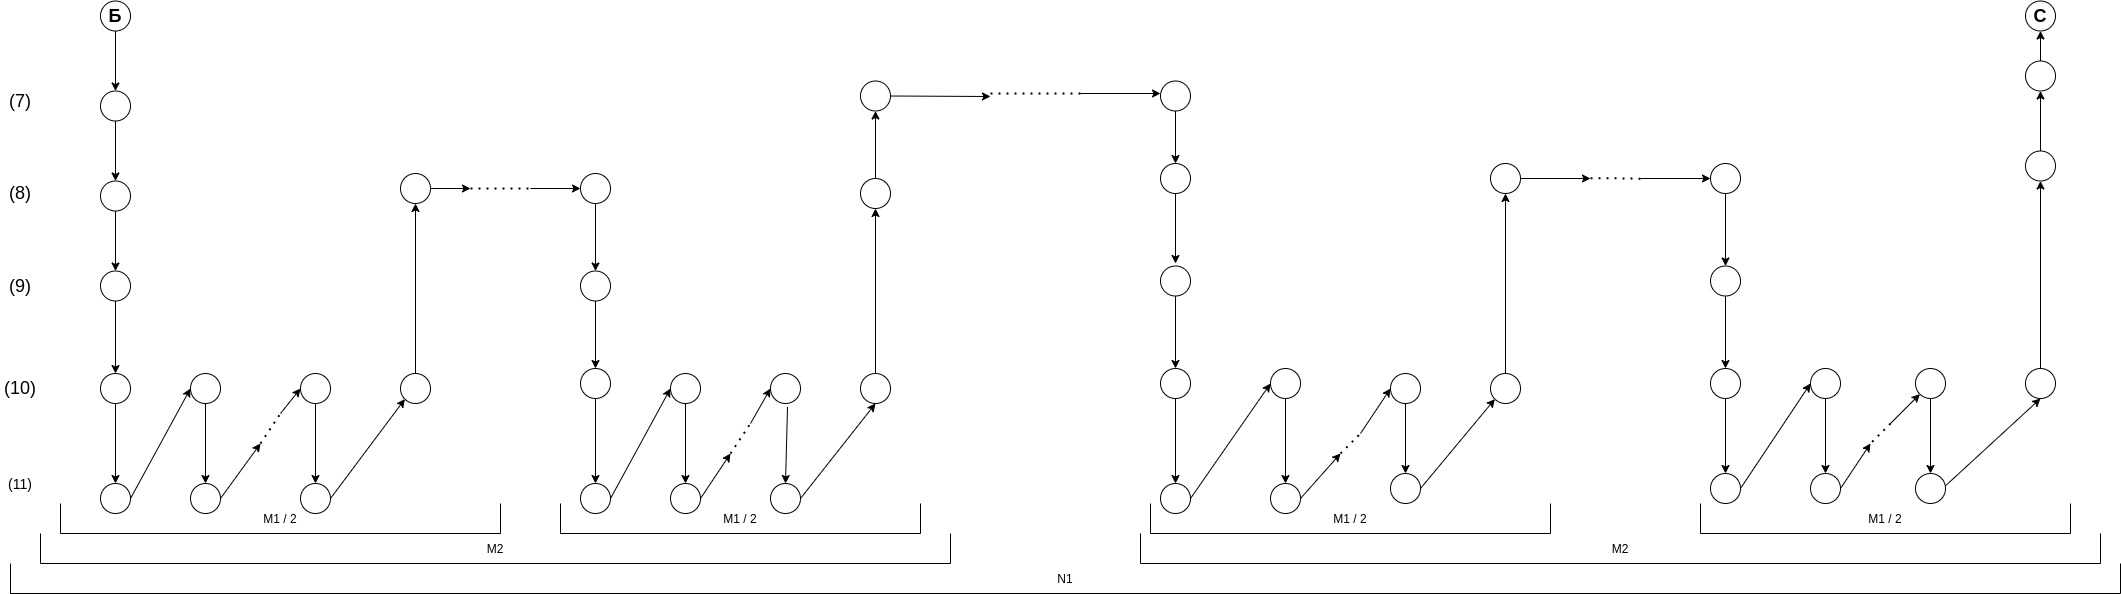
\includegraphics[scale=0.3]{oper_history_2}
	\caption{Операционная история программы. Часть 2}
\end{figure}
\clearpage
\newpage
\begin{figure}[h!]
	\centering
	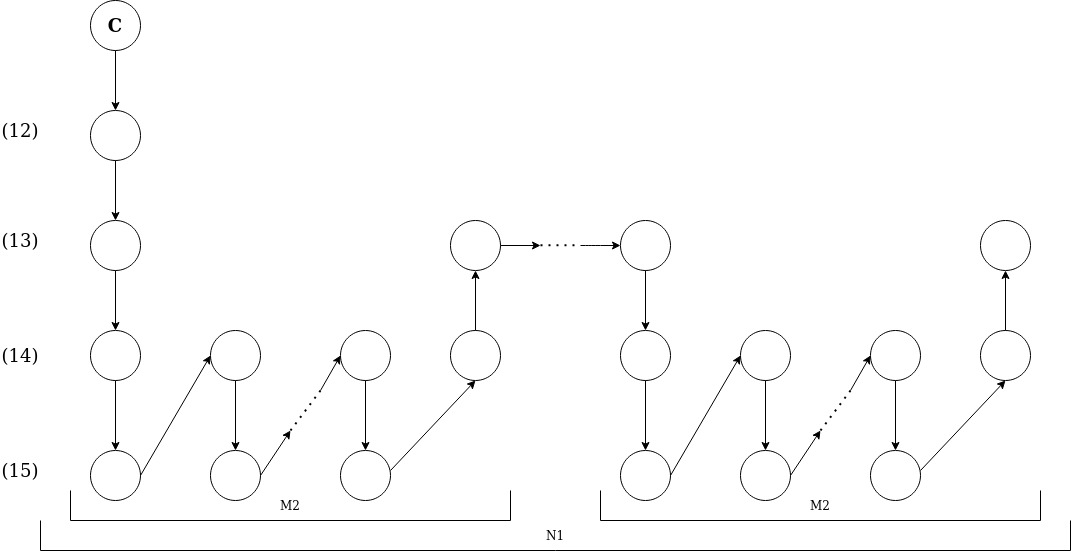
\includegraphics[scale=0.4]{oper_history_3}
	\caption{Операционная история программы. Часть 3}
\end{figure}
\clearpage
\newpage
\subsection{Информационный история программы}
\begin{figure}[h!]
	\centering
	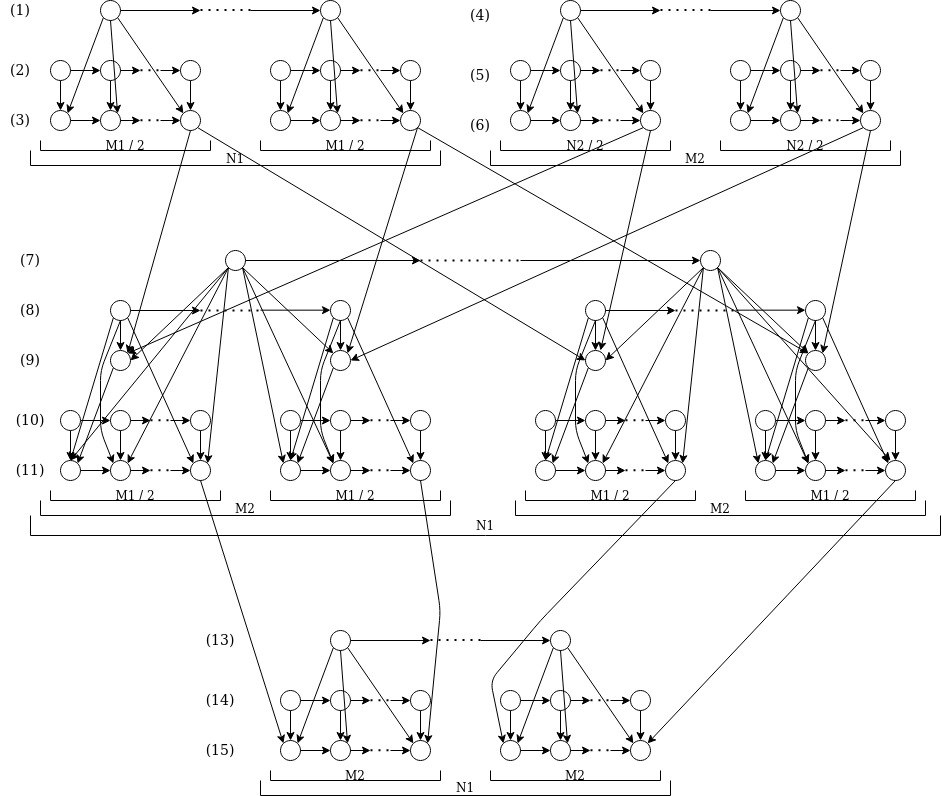
\includegraphics[scale=0.5]{inf_history}
	\caption{Информационный история программы}
\end{figure}


\end{document}